\documentclass[12pt]{article} % use larger type; default would be 10pt

\usepackage{pgfplots}
\usetikzlibrary{calc}
\usetikzlibrary{arrows}
\usetikzlibrary{patterns}
\usetikzlibrary{calc,intersections,through,backgrounds}
\usetikzlibrary{decorations.pathreplacing}
        \newcommand\degree[0]{^{\circ}}
        \newcommand\abs[1]{\left|#1\right|}

\title{Play with TikZ}
\author{Just Us}
%\date{} % Activate to display a given date or no date (if empty),
         % otherwise the current date is printed 

\begin{document}
\maketitle

\section{Law of Sines }





part A: law of sines a circumscribing circle

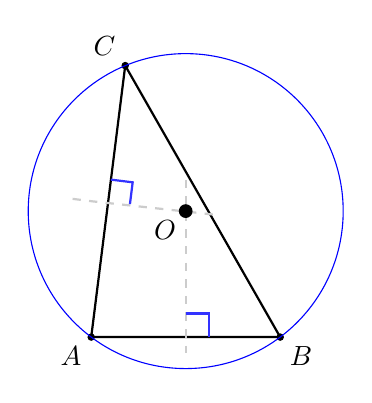
\begin{tikzpicture} [scale=.4]

\coordinate (O) at (0,0);
\coordinate (A) at (-3,-4);
\coordinate (B) at (3,-4);
\coordinate (C) at (-1.92,4.62);

\filldraw (A) circle (.1cm) node[anchor=north east] {$A$};
\filldraw (B) circle (.1cm) node[anchor=north west] {$B$};
\filldraw (C) circle (.1cm) node[anchor=south east] {$C$};

\draw[black,thick] (A)--(B)--(C)--(A);
\draw[gray!40!white, thick, dashed](O)++(0,1) -- (0,-4)--+(0,-.5);
\draw[gray!40!white, thick, dashed](O)++(.862,-.108) -- (-2.96,.31)--++(-.862,.108);
\draw[blue!80!white,thick] (0,-4)++(.75,0)-- ++(0,.75) -- ++(-.75,0);
\draw[blue!80!white,thick] (-2.46,.31) ++(.0864,.6896) -- ++(.6896,-.0864) -- ++(-.0864,-.6896);
\filldraw (O) circle (.2cm) node[anchor=north east] {$O$};

\draw[blue] (O) circle (5);

\end{tikzpicture}
\newline

Kathy's version
\newline

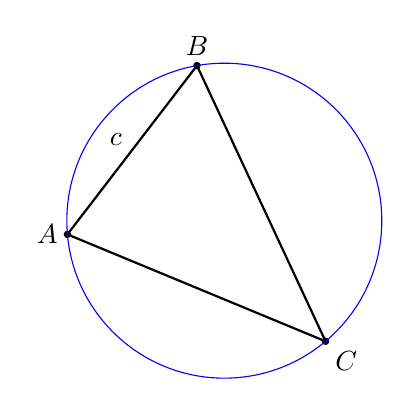
\begin{tikzpicture} [scale=.4]

\coordinate (O) at (0,0);
\coordinate (A) at (185:5);
\coordinate (B) at (100:5);
\coordinate (C) at (-50:5);

\filldraw (A) circle (.1cm) node[anchor= east] {$A$};
\filldraw (B) circle (.1cm) node[anchor=south] {$B$};
\filldraw (C) circle (.1cm) node[anchor=north west] {$C$};

\draw[black,thick] (A)--(B) node[above left, midway, yshift=-2]{$c$};
\draw[black,thick] (B)--(C)--(A);
\draw[blue] (O) circle (5);

\end{tikzpicture}
\newline


Kathy's second
\newline

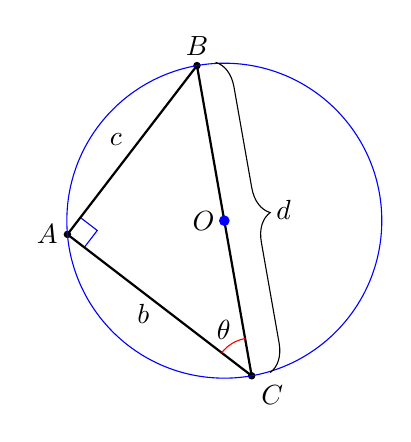
\begin{tikzpicture} [scale=.4]
\coordinate (O) at (0,0);
\coordinate (A) at (185:5);
\coordinate (B) at (100:5);
\coordinate (C) at (-80:5);
\coordinate (p) at ($ (100:5) - (185:5) $);
\coordinate (pp) at ($ (0,0)!1!-90:(p)$);
\filldraw (A) circle (.1cm) node[anchor= east] {$A$};
\filldraw (B) circle (.1cm) node[anchor=south] {$B$};
\filldraw (C) circle (.1cm) node[anchor=north west] {$C$};

\draw[blue] ($ (A) + 0.1*(p)$)--++($ 0.1*(pp) $)--++($ -0.1*(p)$);
\draw[black,thick] (A)--(B) node[above left, midway, yshift=-2]{$c$};
\draw[black,thick] (A)--(C) node[below left, midway, yshift=4]{$b$};
\draw[black,thick] (C)--(B) ;
\draw[red] (C)++(100:1.2) arc (100:142.5:1.2) node[above, midway, xshift=-3, yshift=-2, text=black]{$\theta$};
\draw[blue] (O) circle (5);
\filldraw[blue] (O) circle (.15cm) node[anchor= east, text=black] {$O$};
\draw [decorate,decoration={brace,amplitude=10pt},rotate=190] (-.6,-5) -- (-.6,5) node[right, midway, xshift=.3cm, yshift=.1cm] {$d$};

\end{tikzpicture}
\newline


Kathy's third
\newline

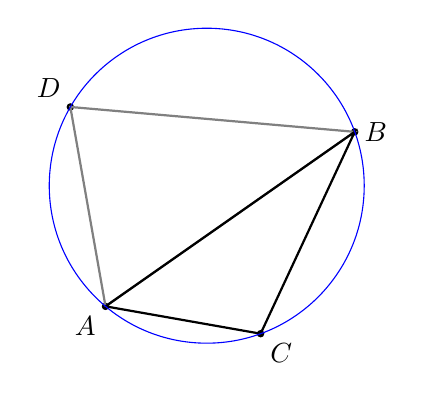
\begin{tikzpicture} [scale=.4]

\coordinate (O) at (0,0);
\coordinate (A) at (230:5);
\coordinate (B) at (20:5);
\coordinate (C) at (-70:5);
\coordinate (D) at (150:5);

\filldraw (A) circle (.1cm) node[anchor= north east] {$A$};
\filldraw (B) circle (.1cm) node[anchor=west] {$B$};
\filldraw (C) circle (.1cm) node[anchor=north west] {$C$};
\filldraw (D) circle (.1cm) node[anchor=south east] {$D$};

\draw[gray,thick] (A)--(B)--(D)--(A) ;
\draw[black,thick] (A)--(B)--(C)--(A) ;
\draw[blue] (O) circle (5);


\end{tikzpicture}
\newline


AMATYC Ignite first
\newline

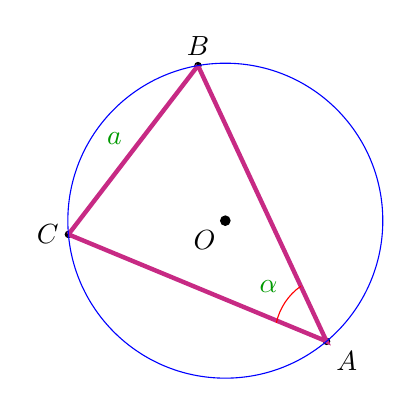
\begin{tikzpicture} [scale=.4]

\coordinate[label=below left:$O$] (O) at (0,0);
\coordinate[label=left:$C$] (C) at (185:5);
\coordinate[label= above:$B$] (B) at (100:5);
\coordinate[label= below right:$A$]  (A) at (-50:5);

\filldraw (A) circle (.1cm);
\filldraw (B) circle (.1cm);
\filldraw (C) circle (.1cm);
\filldraw (O) circle (.15cm);

\draw[magenta!80!black,ultra thick] (C)--(B) node[above left, midway, yshift=-2, text=green!60!black]{$a$};
\draw[magenta!80!black,ultra thick] (B)--(A)--(C);
\draw[blue] (O) circle (5);
%\draw[red,line width=1mm] let \p1 = ($.2*(B) - .2*(C)$) in (C) -- ++(45:({veclen(\x1,\y1)}););
\draw[red] (A)++($.2*(B) - .2*(A)$) let \p1 = ($0.2*(B)-0.2*(A)$) in   arc (125:167.5:({veclen(\x1,\y1)}););
\node[green!60!black, above left, xshift=-.5cm, yshift=.5cm] at (A) {$\alpha$};
\end{tikzpicture}
\newline


Ignite second
\newline

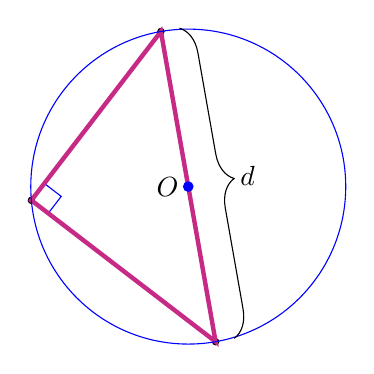
\begin{tikzpicture} [scale=.4]
\coordinate (O) at (0,0);
\coordinate (A) at (185:5);
\coordinate (B) at (100:5);
\coordinate (C) at (-80:5);
\coordinate (p) at ($ (100:5) - (185:5) $);
\coordinate (pp) at ($ (0,0)!1!-90:(p)$);
\filldraw (A) circle (.1cm);
\filldraw (B) circle (.1cm);
\filldraw (C) circle (.1cm);

\draw[blue] ($ (A) + 0.1*(p)$)--++($ 0.1*(pp) $)--++($ -0.1*(p)$);
\draw[magenta!80!black,ultra thick] (A)--(B)--(C)--cycle ;
\draw[blue] (O) circle (5);
\filldraw[blue] (O) circle (.15cm) node[anchor= east, text=black] {$O$};
\draw [decorate,decoration={brace,amplitude=10pt},rotate=190] (-.6,-5) -- (-.6,5) node[right, midway, xshift=.3cm, yshift=.1cm] {$d$};

\end{tikzpicture}
\newline






part B: law of sines a circumscribing circle
\newline

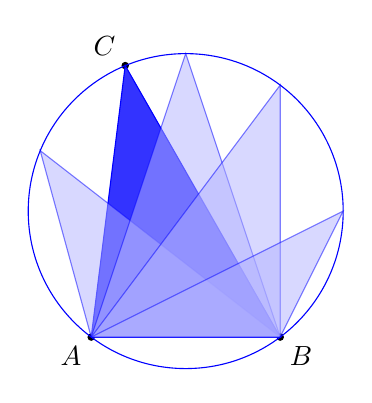
\begin{tikzpicture} [scale=.4]

\coordinate (O) at (0,0);
\coordinate (A) at (-3,-4);
\coordinate (B) at (3,-4);
\coordinate (C) at (-1.92,4.62);
\coordinate (Cp) at (-4.62,1.92);
\coordinate (Cpp) at (0,5);
\coordinate (Cppp) at (3,4);
\coordinate (Cpppp) at (5,0);

\filldraw (O) circle (.1cm) node[anchor=north east] {$O$};
\filldraw (A) circle (.1cm) node[anchor=north east] {$A$};
\filldraw (B) circle (.1cm) node[anchor=north west] {$B$};
\filldraw (C) circle (.1cm) node[anchor=south east] {$C$};

\draw[draw= blue, fill=blue!80!white] (A)--(B)--(C)--(A);
\draw[draw= blue, fill=blue!30!white, opacity=.5] (A)--(B)--(Cp)--(A);
\draw[draw= blue, fill=blue!30!white, opacity=.5] (A)--(B)--(Cpp)--(A);
\draw[draw= blue, fill=blue!30!white, opacity=.5] (A)--(B)--(Cppp)--(A);
\draw[draw= blue, fill=blue!30!white, opacity=.5] (A)--(B)--(Cpppp)--(A);


\draw[blue] (O) circle (5);

\end{tikzpicture}
\newline



\section{Heron's Formula}

angle bisectors of triangle

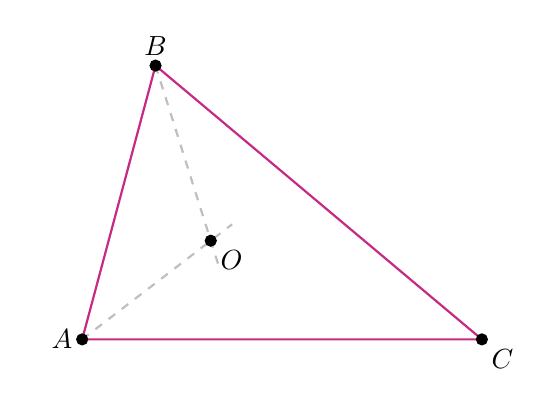
\begin{tikzpicture}
\def\z{1.2}
\def\alp{75};
\def\bet{65};
\def\gam{180-\alp-\bet};
\def\c{3*\z};
%\def\b{\c  * sin(\bet) / sin(\gam) };
\coordinate (A) at (0,0);
\coordinate (B) at (\alp:\c);
\coordinate (C) at ({\c  * sin(\bet) / sin(\gam) },0);

\draw[name path=A--O,lightgray,thick,dashed] (A)--({\alp/2}:2*\z);
\draw[name path=B--O,lightgray,thick,dashed] (B)--++({180+\alp+\bet/2}:2.2*\z);
\path [name intersections={of=A--O and B--O, by=O}];
\draw [name path=O--X, opacity=0]  (O) --++({\alp+90}:2*\z);
\draw [name path=A--B, opacity=0]  (A) --(B);
\path [name intersections={of=O--X and A--B, by=X}];
%\draw[cyan,thick] let \p1 = ($(X)-(O)$) in  (O) circle ({veclen(\x1,\y1)});
%\draw[green!80!black,thick] (O)--(X);
%\draw[lightgray, thick, dashed] (O)--(C);
\draw[magenta!80!black,thick] (A)--(B)--(C)--(A);
\filldraw (O) circle (.7mm) node[anchor=north west] {$O$};
\filldraw (A) circle (.7mm) node[anchor=east] {$A$};
\filldraw (B) circle (.7mm) node[anchor=south] {$B$};
\filldraw (C) circle (.7mm) node[anchor=north west] {$C$};
%\filldraw (X) circle (.7mm) node[anchor=south east] {$P$};


\end{tikzpicture}
\newline

inscribed circle

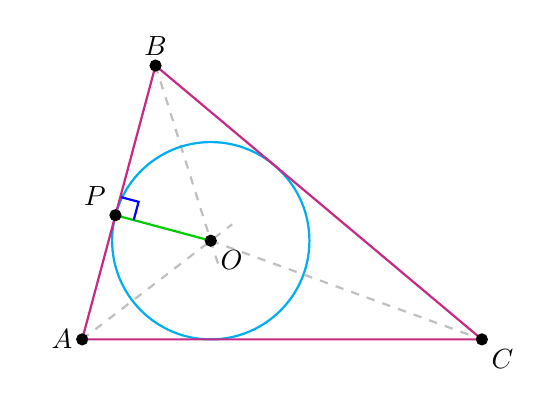
\begin{tikzpicture}
\def\z{1.2}
\def\alp{75};
\def\bet{65};
\def\gam{180-\alp-\bet};
\def\c{3*\z};
%\def\b{\c  * sin(\bet) / sin(\gam) };
\coordinate (A) at (0,0);
\coordinate (B) at (\alp:\c);
\coordinate (C) at ({\c  * sin(\bet) / sin(\gam) },0);

\draw[name path=A--O,lightgray,thick,dashed] (A)--({\alp/2}:2*\z);
\draw[name path=B--O,lightgray,thick,dashed] (B)--++({180+\alp+\bet/2}:2.2*\z);
\path [name intersections={of=A--O and B--O, by=O}];
\draw [name path=O--X, opacity=0]  (O) --++({\alp+90}:2*\z);
\draw [name path=A--B, opacity=0]  (A) --(B);
\path [name intersections={of=O--X and A--B, by=X}];
\draw[cyan,thick] let \p1 = ($(X)-(O)$) in  (O) circle ({veclen(\x1,\y1)});
\draw[green!80!black,thick] (O)--(X);
\draw[blue,thick] (X)++(\alp:{.2*\z})--++(\alp-90:{.2*\z})--++(\alp-180:{.2*\z});
\draw[lightgray, thick, dashed] (O)--(C);
\draw[magenta!80!black,thick] (A)--(B)--(C)--(A);
\filldraw (O) circle (.7mm) node[anchor=north west] {$O$};
\filldraw (A) circle (.7mm) node[anchor=east] {$A$};
\filldraw (B) circle (.7mm) node[anchor=south] {$B$};
\filldraw (C) circle (.7mm) node[anchor=north west] {$C$};
\filldraw (X) circle (.7mm) node[anchor=south east] {$P$};


\end{tikzpicture}
\newline

area =  radius * semiperimeter

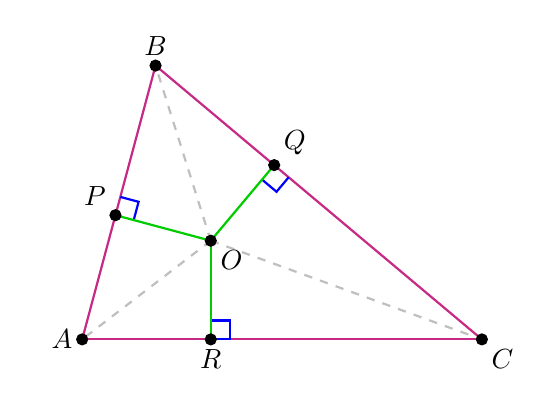
\begin{tikzpicture}
\def\z{1.2}
\def\alp{75};
\def\bet{65};
\def\gam{180-\alp-\bet};
\def\c{3*\z};
%\def\b{\c  * sin(\bet) / sin(\gam) };
\coordinate (A) at (0,0);
\coordinate (B) at (\alp:\c);
\coordinate (C) at ({\c  * sin(\bet) / sin(\gam) },0);

\draw[name path=A--O, opacity=0] (A)--({\alp/2}:2*\z);
\draw[name path=B--O, opacity=0] (B)--++({180+\alp+\bet/2}:2*\z);
\path [name intersections={of=A--O and B--O, by=O}];
\draw [name path=O--X, opacity=0]  (O) --++({\alp+90}:2*\z);
\draw [magenta!80!black,name path=A--B,thick]  (A) --(B);
\path [name intersections={of=O--X and A--B, by=X}];
\draw[blue,thick] (X)++(\alp:{.2*\z})--++(\alp-90:{.2*\z})--++(\alp-180:{.2*\z});
\draw[green!80!black,thick] (O)--(X);
\draw [name path=O--Y, opacity=0]  (O) --++({90-(\gam)}:2*\z);
\draw [magenta!80!black,name path=B--C,thick]  (B) --(C);
\path [name intersections={of=O--Y and B--C, by=Y}];
\draw [name path=O--Z, opacity=0]  (O) --++(0,-1.5*\z);
\draw [magenta!80!black,name path=A--C,thick]  (A) --(C);
\path [name intersections={of=O--Z and A--C, by=Z}];
\draw[blue,thick] (Y)++({-90-(\gam)}:.2*\z)--++({-(\gam)}:.2*\z)--++({90-(\gam)}:.2*\z);
\draw[blue,thick] (Z) rectangle ++({.2*\z},{.2*\z});
\draw[green!80!black,thick] (O)--(Y);
\draw[green!80!black,thick] (O)--(Z);
\draw[lightgray,thick,dashed] (O)--(A);
\draw[lightgray,thick,dashed] (O)--(B);
\draw[lightgray,thick,dashed] (O)--(C);
\filldraw (O) circle (.7mm) node[anchor=north west] {$O$};
\filldraw (A) circle (.7mm) node[anchor=east] {$A$};
\filldraw (B) circle (.7mm) node[anchor=south] {$B$};
\filldraw (C) circle (.7mm) node[anchor=north west] {$C$};
\filldraw (X) circle (.7mm) node[anchor=south east] {$P$};
\filldraw (Y) circle (.7mm) node[anchor=south west] {$Q$};
\filldraw (Z) circle (.7mm) node[anchor=north] {$R$};

%\draw[black,thick] (A)--(B)--(C)--(A);
\end{tikzpicture}
\newline

triangle lengths labeled

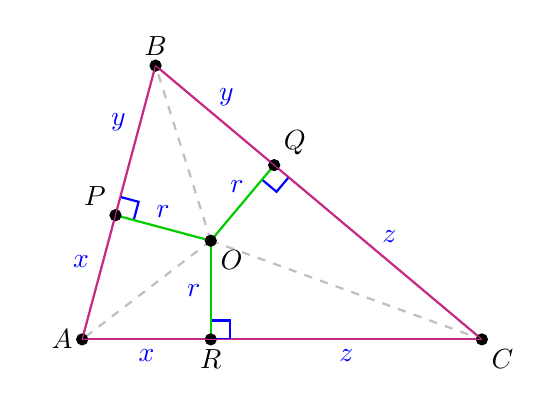
\begin{tikzpicture}
\def\z{1.2}
\def\alp{75};
\def\bet{65};
\def\gam{180-\alp-\bet};
\def\c{3*\z};
%\def\b{\c  * sin(\bet) / sin(\gam) };
\coordinate (A) at (0,0);
\coordinate (B) at (\alp:\c);
\coordinate (C) at ({\c  * sin(\bet) / sin(\gam) },0);

\draw[name path=A--O, opacity=0] (A)--({\alp/2}:2*\z);
\draw[name path=B--O, opacity=0] (B)--++({180+\alp+\bet/2}:2*\z);
\path [name intersections={of=A--O and B--O, by=O}];
\draw [name path=O--X, opacity=0]  (O) --++({\alp+90}:2*\z);
\draw [magenta!80!black,name path=A--B,thick]  (A) --(B);
\path [name intersections={of=O--X and A--B, by=X}];
\draw[blue,thick] (X)++(\alp:{.2*\z})--++(\alp-90:{.2*\z})--++(\alp-180:{.2*\z});
\draw[green!80!black,thick] (O)--(X) node[above, midway, text=blue]{$r$};
\draw [name path=O--Y, opacity=0]  (O) --++({90-(\gam)}:2*\z);
\draw [magenta!80!black,name path=B--C,thick]  (B) --(C);
\path [name intersections={of=O--Y and B--C, by=Y}];
\draw [name path=O--Z, opacity=0]  (O) --++(0,-1.5*\z);
\draw [magenta!80!black,name path=A--C,thick]  (A) --(C);
\path [name intersections={of=O--Z and A--C, by=Z}];
\draw[blue,thick] (Y)++({-90-(\gam)}:.2*\z)--++({-(\gam)}:.2*\z)--++({90-(\gam)}:.2*\z);
\draw[blue,thick] (Z) rectangle ++({.2*\z},{.2*\z});
\draw[green!80!black,thick] (O)--(Y) node[above, midway, xshift=-2, text=blue]{$r$};
\draw[green!80!black,thick] (O)--(Z) node[left, midway, text=blue]{$r$};
\draw[lightgray,thick,dashed] (O)--(A);
\draw[lightgray,thick,dashed] (O)--(B);
\draw[lightgray,thick,dashed] (O)--(C);
\filldraw (O) circle (.7mm) node[anchor=north west] {$O$};
\filldraw (A) circle (.7mm) node[anchor=east] {$A$};
\filldraw (B) circle (.7mm) node[anchor=south] {$B$};
\filldraw (C) circle (.7mm) node[anchor=north west] {$C$};
\filldraw (X) circle (.7mm) node[anchor=south east] {$P$};
\filldraw (Y) circle (.7mm) node[anchor=south west] {$Q$};
\filldraw (Z) circle (.7mm) node[anchor=north] {$R$};
\draw [magenta!80!black]  (A) --(X) node[above left, midway, text=blue] {$x$};
\draw [magenta!80!black]  (A) --(Z) node[below, midway, text=blue] {$x$};
\draw [magenta!80!black]  (B) --(X) node[above left, midway, text=blue] {$y$};
\draw [magenta!80!black]  (B) --(Y) node[above right, xshift=-2, midway, text=blue] {$y$};
\draw [magenta!80!black]  (C) --(Y) node[above right, xshift=-2, midway, text=blue] {$z$};
\draw [magenta!80!black]  (C) --(Z) node[below, midway, text=blue] {$z$};

%\draw[black,thick] (A)--(B)--(C)--(A);
\end{tikzpicture}
\newline

Heron

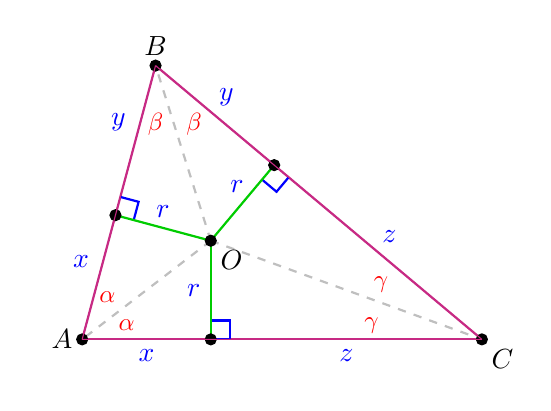
\begin{tikzpicture}
\def\z{1.2}
\def\alp{75};
\def\bet{65};
\def\gam{180-\alp-\bet};
\def\c{3*\z};
\coordinate (A) at (0,0);
\coordinate (B) at (\alp:\c);
\coordinate (C) at ({\c  * sin(\bet) / sin(\gam) },0);

\draw[name path=A--O, opacity=0] (A)--({\alp/2}:2*\z);
\draw[name path=B--O, opacity=0] (B)--++({180+\alp+\bet/2}:2*\z);
\path [name intersections={of=A--O and B--O, by=O}];
\draw [name path=O--X, opacity=0]  (O) --++({\alp+90}:2*\z);
\draw [magenta!80!black,name path=A--B,thick]  (A) --(B);
\path [name intersections={of=O--X and A--B, by=X}];
\draw[blue,thick] (X)++(\alp:{.2*\z})--++(\alp-90:{.2*\z})--++(\alp-180:{.2*\z});
\draw[green!80!black,thick] (O)--(X) node[above, midway, text=blue]{$r$};
\draw [name path=O--Y, opacity=0]  (O) --++({90-(\gam)}:2*\z);
\draw [magenta!80!black,name path=B--C,thick]  (B) --(C);
\path [name intersections={of=O--Y and B--C, by=Y}];
\draw [name path=O--Z, opacity=0]  (O) --++(0,-1.5*\z);
\draw [magenta!80!black,name path=A--C,thick]  (A) --(C);
\path [name intersections={of=O--Z and A--C, by=Z}];
\draw[blue,thick] (Y)++({-90-(\gam)}:.2*\z)--++({-(\gam)}:.2*\z)--++({90-(\gam)}:.2*\z);
\draw[blue,thick] (Z) rectangle ++({.2*\z},{.2*\z});
\draw[green!80!black,thick] (O)--(Y) node[above, xshift=-2, midway, text=blue]{$r$};
\draw[green!80!black,thick] (O)--(Z) node[left, midway, text=blue]{$r$};
\draw[lightgray,thick,dashed] (O)--(A);
\draw[lightgray,thick,dashed] (O)--(B);
\draw[lightgray,thick,dashed] (O)--(C);
\filldraw (O) circle (.7mm) node[anchor=north west] {$O$};
\filldraw (A) circle (.7mm) node[anchor=east] {$A$};
\filldraw (B) circle (.7mm) node[anchor=south] {$B$};
\filldraw (C) circle (.7mm) node[anchor=north west] {$C$};
\filldraw (X) circle (.7mm);
\filldraw (Y) circle (.7mm);
\filldraw (Z) circle (.7mm);
\node[above right, xshift=3, yshift=10, text=red, scale=.9] at (A) {$\alpha$};
\node[above right, xshift=10, text=red, scale=.9] at (A)  {$\alpha$};
\node[below, yshift=-14, text=red, scale=.9] at (B)  {$\beta$};
\node[below right, xshift=8, yshift=-14, text=red, scale=.9] at (B)  {$\beta$};
\node[above left, xshift=-\z cm, yshift=-1, text=red, scale=.9] at (C)  {$\gamma$};
\node[above left, xshift=-0.9*\z cm, yshift=0.4*\z cm, text=red, scale=.9] at (C)  {$\gamma$};
\draw [magenta!80!black]  (A) --(X) node[above left, midway, text=blue] {$x$};
\draw [magenta!80!black]  (A) --(Z) node[below, midway, text=blue] {$x$};
\draw [magenta!80!black]  (B) --(X) node[above left, midway, text=blue] {$y$};
\draw [magenta!80!black]  (B) --(Y) node[above right, xshift=-2, midway, text=blue] {$y$};
\draw [magenta!80!black]  (C) --(Y) node[above right, xshift=-2, midway, text=blue] {$z$};
\draw [magenta!80!black]  (C) --(Z) node[below, midway, text=blue] {$z$};

%\draw[black,thick] (A)--(B)--(C)--(A);
\end{tikzpicture}
\newline







\end{document}
